\documentclass[10pt,twocolumn]{article}
%% Welcome to Overleaf!
%% If this is your first time using LaTeX, it might be worth going through this brief presentation:
%% https://www.overleaf.com/latex/learn/free-online-introduction-to-latex-part-1

%% Researchers have been using LaTeX for decades to typeset their papers, producing beautiful, crisp documents in the process. By learning LaTeX, you are effectively following in their footsteps, and learning a highly valuable skill!

%% The \usepackage commands below can be thought of as analogous to importing libraries into Python, for instance. We've pre-formatted this for you, so you can skip right ahead to the title below.

%% Language and font encodings
\usepackage[spanish,english]{babel}
\usepackage[utf8x]{inputenc}
\usepackage[T1]{fontenc}

%% Sets page size and margins
\usepackage[a4paper,top=2cm,bottom=2cm,left=2cm,right=2cm,marginparwidth=2cm]{geometry}

%% Useful packages
\usepackage{amsmath}
\usepackage{graphicx}
\usepackage[colorinlistoftodos]{todonotes}
\usepackage[colorlinks=true, allcolors=blue]{hyperref}
\usepackage{float}

%% Title
\title{
		%\vspace{-1in} 	
		\usefont{OT1}{bch}{b}{n}
		\normalfont \normalsize \textsc{CSE-4111 Artificial Intelligence Lab} \\ [10pt]
		\huge Constraint Satisfaction Problem : Arc Consistency Algorithms \\
}

\usepackage{authblk}
\author[0]{\textbf{Saif Mahmud}\\
		4th Year 1st Semester, Roll : SH - 054\\}


\begin{document}
\maketitle

\selectlanguage{english}
\begin{abstract}
Constraint Satisfaction Problem (CSP) is defined as a triple $ P = (X, D, C) $ where $ X = \{1,...,n\} $ is a set of variables. Each variable $ X_{i} ∈ X $ has a finite domain $ D_{i} ∈ D $ of values that can be assigned to it. Arc consistency is defined as $ X_{i} $ is arc-consistent with respect to another variable $ X_{j} $ if for every value in the current domain $ D_{i} $ there is some value in the domain $ D_{j} $ that satisfies the binary constraint on the arc $ (X_{i} , X_{j}) $. A CSP is arc consistent (AC) if and only if every variable is arc consistent. Arc Consistency is achieved through removing arc inconsistent values until complete consistency or a failure is obtained. In this regard, there are 4 (four) algorithms within the scope of this experiment attaining the goal of removing arc inconsistency from CSPs and they are namely \textit{AC - 1, AC - 2, AC - 3, and AC - 4}.
\end{abstract}

\section{Proposed Approach}

\subsection{Implementation of Algorithms}
The Constraint Satisfaction Problem (CSP) is defined as a tuple of Variables(X), Domains(D) and Constraints(C). Here, in the approach of solving the proposed problem, I have implemented CSP as a Python class with the constructor defining X, D and C. In this regard, Variables(X) is a list of strings denoting the names of the variables, Domains(D) is defined as a dictionary with the variable as key and a list of integers as value and Constraints(C) is implemented as a dictionary with a tuple of variables denoting the edge between two nodes and in the value, a logical relationship as binary constraint. The algorithms for obtaining arc consistency is implemented along with the auxiliary functions within the scope of this CSP class. The outcome of the Arc Consistency(AC) algorithms is the reduced domain for each variable satisfying the defined binary constraints. Hence, after executing the \textit{AC-1/2/3/4} functions, the program will eliminate the inconsistent values from the list defined in the Domains(D) dictionary for each variable. If the constraint graph becomes partially consistent in the way of maintaining arc consistency, then the domain of particular variable will become empty as no value in the domain can satisfy the binary constraint. As a result, we function will return with a \textit{False} flag.

\subsection{Input Graph Generation}
The constraint graph is generated with a mindset to vary the defining tuples of constraint satisfaction problem. The number of nodes is increased in order to determine the performance bottleneck dependency upon the number of variables in constraint graph. The number of edges indicates the density of constraint graph. The number of edges has been picked proportional to the number of nodes in order obtain consistent result for evaluation metric. If the constraint graph is sparse, it implies that fewer binary relationship as constraints is imposed. The size of the domain has been made both fixed and random within a range in order to predict the dependency of performance on domain size. I have created a pool of binary constraints as per the description of the constraint satisfaction problem. The constraints are assigned among two variables through picking one form the pool and coupling with the edge or arc. The constraint graph generator program generates the parameter for CSP in \textit{.txt} files which are used as arguments for instantiating the CSP object and running arc consistency algorithms.
\section{Result of the Experiment}

\subsection{Performance Analysis}
In Figure \ref{fig:01}, the performance graph indicates the elapsed time with the increasing number of nodes. It can be inferred from the graph that, the number of nodes adds complexity to execution time of the arc consistency algorithms. Moreover, the performance of AC4 algorithms degrades drastically than others. On the other hand, AC3 maintains better execution time than other algorithms in spite of the increment in the number of nodes. 
\begin{figure}[H]
	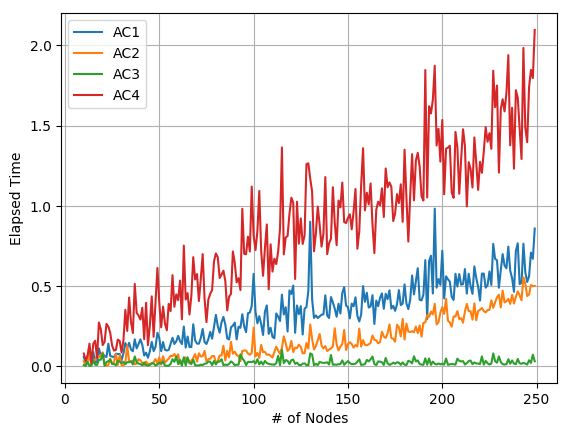
\includegraphics[width = \columnwidth, height = 6cm]{fig1}
	\caption{Elapsed Time with respect to Number of Nodes where Edges = 2 * Nodes}
	\label{fig:01}
\end{figure}
If the number of edges increased with the same number of nodes then execution time vs. number of nodes graph in Figure \ref{fig:02} fluctuates more due to the increased probability of inconsistency than sparse graph with fewer constraints.   
\begin{figure}[H]
	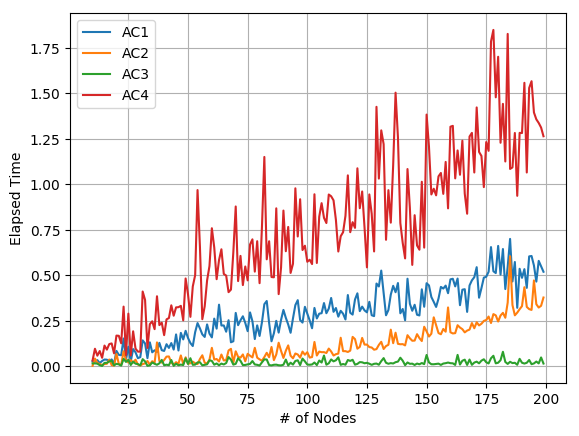
\includegraphics[width = \columnwidth, height = 6cm]{fig2}
	\caption{Elapsed Time with respect to Number of Nodes where Edges = 3 * Nodes}
	\label{fig:02}
\end{figure}
In case of the result described in Figure \ref{fig:01} and \ref{fig:02}, the domain size was maintained within the range of $ [25, 50] $.We can see in Figure \ref{fig:03} that if the domain size is increased and the domains of each variable consist of discrete integer values from the same specified range then the performance of AC2 and AC3 with respect to time complexity almost aligns, but the performance of AC1 and AC4 remains more or less same. If the domain size is relatively larger, it is less probable that the constraint graph will move forward to partial consistency. Therefore, it can be inferred that the vulnerability of performance depends upon the consistency characteristics of the CSP. 
\begin{figure}[H]
	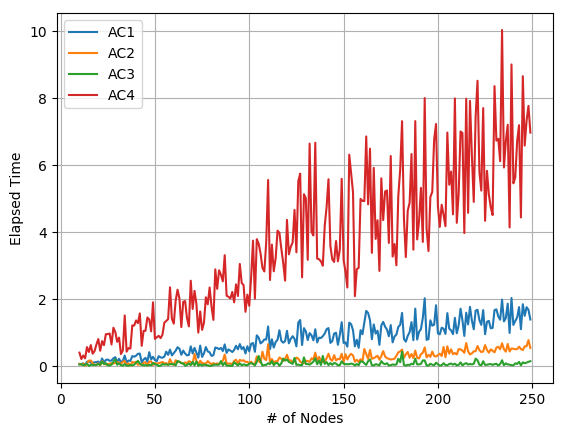
\includegraphics[width = \columnwidth, height = 6cm]{fig5}
	\caption{Elapsed Time with respect to Number of Nodes where Domain Size = [25, [75, 125]]}
	\label{fig:03}
\end{figure}
If we eliminate the certain scenario of inconsistency from the constraint graph and then we obtain the Figure \ref{fig:04}. In this case, I have taken the elapsed time of the graphs only which are consistent and found that AC1, AC2 and AC2 performs nearly identical. On the other hand, AC4 still shows some exponential nature in elapsed time even with the consistent graphs.
\begin{figure}[H]
	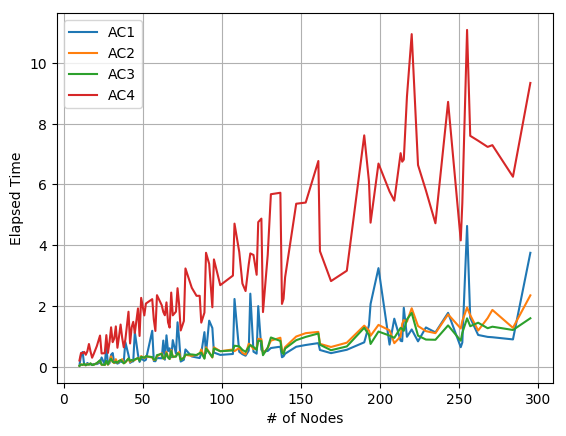
\includegraphics[width = \columnwidth, height = 6cm]{fig6}
	\caption{Elapsed Time with respect to Number of Nodes where All CSP are consistent}
	\label{fig:04}
\end{figure}

\subsection{ANOVA with Tukey HSD}
I have taken the data of $ k = 4 $ independent treatments where A, B, C and D are described as per the elapsed time of AC1, AC2, AC3 and AC4 on the constraint graphs with increasing number of nodes or variables.

In case of the constraint graphs with amalgamation of consistent and inconsistent ones, the significance test ANOVA with Tukey HSD yields statistical significance in each case.  
\begin{figure}[H]
	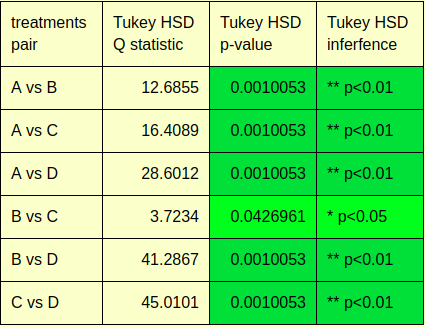
\includegraphics[width = \columnwidth, height = 6cm]{anova_1}
	\caption{ANOVA Test Result}
	\label{fig:05}
\end{figure}
On the other hand, if we consider only the consistent constraint graph for performance comparison then the following ANOVA with Tukey HSD in Figure \ref{fig:06}. Here, AC1 is statistically insignificant with respect to AC2 and AC3 as well as AC2 is insignificant with AC3.
\begin{figure}[H]
	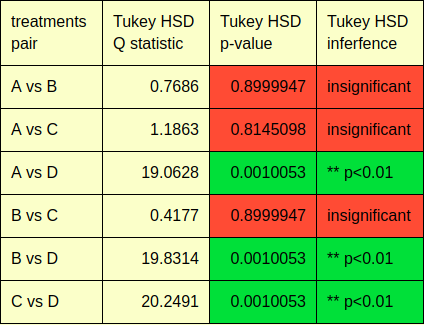
\includegraphics[width = \columnwidth, height = 6cm]{anova_2}
	\caption{ANOVA Test Result (Consistent)}
	\label{fig:06}
\end{figure}
The details result of ANOVA with HSD Tukey is given in the appendix for further reference.

\section{Discussion}
I have inferred the following findings through performing this experiment on Arc Consistency algorithms :
\begin{itemize}
	\item AC3 algorithm is computationally the most efficient in comparison with other algorithms. Though it pushes the edges of any specific node on the event of modification in its domain in order to obtain consistency, it has the early termination feature which plays well to discard the algorithm as soon as any of the node's domain become empty.
	\item AC4 has yielded worst result according to my experimental setting. But it should not be considered as a concluding proposition because there are some bottlenecks of using python built-in data structures. According to my opinion, in many cases python data structures have caused execution time overhead which is severe in case of AC4 implementation.
	\item It is a natural phenomenon that with the increase in number of nodes the elapsed time of every algorithm increases in varied proportion. The cause of this relationship can be conceived as the nodes increases the number of variables for which arc consistency should be obtained.
	\item The number of edges in a constraint graph is an indicator of imposed constraints on the domain. If we increase the number of edges then there is more constraints to satisfy. Therefore, the probability of partial consistency increases with the density of graph. For example, if we consider a sparse graph with approximately number of edges as twice as the nodes and a dense one with thrice, it is apparent that the arc consistency algorithm performs better on the sparse graph due to fewer constraints.
	\item The more explicit and tight constraint networks are, the more restricted is the search space of partial solutions. Therefore, if we impose tight constraints then it is more likely that any entity in the domain set cannot satisfy the constraints and thus become inconsistent. In case of this experiment, I have eliminated the constraints like $ x == y $ in case of non-intersecting domains because it was causing domains to become empty and hence partial consistent. It should be noted that the definition of together constraints varied on the basis of characteristics of domain, for example intersecting and non-intersecting domains or continuous and discrete domains.
	\item Node consistency with respect to global constraint can be achieved if the same constraint is included in all the edges. 
	\item We can refer to a lemma that checking whether a network or constraint graph is arc-consistent requires at most $ e * k^{2} $ operations where $ e $ is the number of its binary constraints imposed and $ k $ is an upper bound of its domain sizes. So, the inference obtained from the experiment indicates that number of edges and size of domains plays vital role as performance bottleneck because each algorithm incorporates revision of domains.
	\item When all the graphs in consideration are consistent then the early termination becomes obsolete and so the difference between the performance shrinks. But due to the implementation with complex python data structure AC4 still shows a little bit exponential nature.
\end{itemize}

\end{document}
